% !TEX program = xelatex
\documentclass{amsart}
\usepackage{graphicx} % Required for inserting images
\usepackage{amsthm, amsmath, amssymb, amsfonts} % general mathmode commands
\usepackage{bm} % for \bm
\usepackage{stmaryrd} % for \nnearrow
\usepackage{cancel} % for \cancel
\usepackage{breqn} % automatic line breaks in equations
\usepackage[margin=2.5cm]{geometry} % for page layout
\usepackage{cancel} % for \cancel
\usepackage{algorithm2e} % for algorithms
\usepackage{bbm} % for \mathbbm{1}
\usepackage{mathtools} % for \coloneq
\usepackage{hyperref}
\usepackage{nicefrac}
\usepackage{float}
\usepackage{polyglossia}
\usepackage{biblatex}
\usepackage{lipsum}
\usepackage{placeins}
\usepackage{booktabs}
\usepackage{xcolor,colortbl}
\usepackage{makecell}
\RestyleAlgo{ruled}

% \new theorems definition
\theoremstyle{plain}
\newtheorem{theorem}{Theorem}
\newtheorem{corollary}[theorem]{Corollary}
\newtheorem{lemma}[theorem]{Lemma}
\newtheorem{claim}[theorem]{Claim}
\newtheorem{proposition}[theorem]{Proposition}

\theoremstyle{definition}
\newtheorem{definition}[subsection]{Definition}

\theoremstyle{definition}
\newtheorem{example}[subsection]{Example}
\newtheorem{conjecture}[subsection]{Conjecture}

\theoremstyle{remark}
\newtheorem{remark}[subsection]{Remark}

\addbibresource{refs.bib}
% \newcommand
\DeclareMathOperator*{\argmax}{argmax}
\DeclareMathOperator{\err}{Err}
\DeclareMathOperator{\softmax}{softmax}
\DeclareMathOperator{\esscher}{\mathfrak{H}}
\newcommand{\diff}{\mathrm{d}}

% Language settings
\setdefaultlanguage{english}
\setotherlanguage{hebrew}
\newfontfamily\hebrewfont[Script=Hebrew]{Arial}
\title{Research Proposal}
\author{Mark Sverdlov}
\date{December 2025}

\begin{document}

\begin{titlepage}
    \begin{center}
        \vspace*{1cm}

        \Large{Risk Measure Bounds under Partial Distributional Information}

        \Large{\texthebrew{חסמים של מידות סיכון תחת מידע חלקי על ההתפלגות}}

        Mark Sverdlov \\
        ID:\@ 323454710
        \vspace{0.8cm} \\
        Advisors: Prof.\@ Simcha Haber, Dr.\@ Rom Aviv
        \vspace{0.8cm} \\
        Department of Mathemetics, Bar Ilan University \\
        May 2026
    \end{center}
\end{titlepage}

\section{Introduction}
\subsection{Historical Background}
Catastrophic events, like hurricanes or earthquakes, pose a unique risk profile for insurers and reinsurers, due to their tendency to affect whole industries and sectors in tandem. These risks were realized in 1992, when Hurricane Andrew struck Florida and the Gulf Coast, inflicting \$27 billion in damages, of which \$15.5 billion was covered by insurance~\cite{chicago-history}. This event led to the failure of eight insurance companies, and pushed others to the brink of insolvency.
Indeed, losses of that scale are insufferable for individual establishments or hedge funds. This fact leads naturally to looking for solutions in the capital market, which represents the economic power of the general public.
Hence, this turn of events eventually culminated in the invention of the financial machinery of a CAT bond, which is a security that pays the issuer when a predefined disaster risk is realized. The first CAT bonds were issued in 1997, giving insurers access to broader financial markets, and offering institutional investors an opportunity to earn an attractive return on investment uncorrelated with the returns of other financial instruments.

From 1997 to 2005, CAT bond issuance was steady, averaging \$1.2 billion annually, but CAT bonds gained popularity as a means of diversifying risk after the insured losses from Hurricane Katrina, culminating in \$25.4 billion in CAT bonds issued this year (2025)~\cite{artemis}. This puts CAT bonds as a valuable and interesting financial instrument, garnering attention both from academics and practitioners.

\subsection{Literature Background}
As financial instruments, the main objective of research on CAT bonds and ILS is pricing their risk, i.e.\ creating a model that is able to calculate the spread of the bond yield over the risk-free yield given its conditions, the economic environment, and past data. This objective is complicated by the existence of differently structured bonds with different insured underlying risks. A model built to tackle pricing for a relatively simple case is~\cite{zimbidis-et-al}, where a model is constructed to price non-indemnity CAT bonds over earthquakes in the broader area of Greece. The modeling is done in two stages: first, a probability distribution of the maximal earthquake intensity in a time period is fitted over historical data using tools from Extreme Value Theory; then, this distribution is set in a classical formula to price a bond given an economic environment (risk-free interest rate, etc.). A more abstract approach is taken by Wang~\cite{wang}, where the premise is that the distribution of the underlying event (loss due to some disaster) is given by physical considerations, either as an output of some catastrophic modeling program (based on historical data) or an event-loss table stating the probability and financial loss of different events. To price the bond, we transform the probability measure to load the risks associated with the bond using a probability transformation, resulting in a `price-curve'. Observing that most of the information about a loss distribution is contained in the \textit{attachment probability}, \textit{expected loss}, and \textit{exhaustion probability},~\cite{rom} develops a framework to approximate a loss exceedance probability curve using these three numbers, utilizing tools from Extreme Value Theory. 
\subsection{Definitions}
Our main object of study is the \textit{excess of loss} layer within a reinsurance program. We model it with a random variable \(L\) bounded in \(\left[0,\,1\right]\), which we call the \emph{loss} variable, defined over some probability space \(\left(\Omega,\,\mathcal{F}, P\right)\). \(L = 0\) represents the event when the layer is not triggered. \(L = 1\) represents the event when the layer is fully exhausted, and \(0 < L < 1\) denotes the proportional payout out of the total layer. We henceforth define a few terms to more easily present our proposed problem and preliminary results:

\begin{definition}[Attachment Probability]
    The attachment probability is the probability that the layer is triggered. We denote:
    \begin{equation*}
        p_{\text{attachment}} = P \left(L > 0\right)
    \end{equation*}
\end{definition}
\begin{definition}[Exhaustion Probability]
    The exhaustion probability is the probability that the layer is exhausted. We denote:
    \begin{equation*}
        p_{\text{exhaustion}} = P \left(L = 1\right)
    \end{equation*}
\end{definition}
\begin{definition}[Expected Loss]
    The expected loss is the expectation of the loss variable, and is denoted by \(\mathrm{E}L\).
\end{definition}
\begin{definition}[Loss Exceedance Curve]
   The loss exceedance curve is the function:
   \begin{align*}
       s_{L}: \ \left[0,\,1\right] &\rightarrow \left[0,\infty\right) \\
                                 x &\mapsto P \left(L > x\right)
   \end{align*}
   which denotes the probability that the loss exceeds a value \(x\).
\end{definition}
\begin{definition}[\(\alpha\)-quantile]
   Given some \(\alpha \in \left[0,\,1\right]\), we define:
   \begin{equation*}
       q_{\alpha} \left(L\right) = \inf \left\{q \in \left[0,\,1\right] \mid P \left(L \leq q\right) \geq \alpha\right\}
   \end{equation*}
   where by convention we define \(\inf \emptyset = 0\).
\end{definition}
\begin{definition}[Value at Risk]
    Given some confidence level \(\alpha \in \left(0,\,1\right)\), we define the value at risk with confidence level \(\alpha\) to be:
    \begin{equation*}
        \text{VaR}_{\alpha} L = \inf \left\{V \in \left[0,\,1\right] \mid P \left(L > V\right) \leq 1 - \alpha\right\} = q_{\alpha}\left(L\right)
    \end{equation*}
   where by convention we define \(\inf \emptyset = 0\).
\begin{remark}
    For all \(\alpha \in \left[0,\,1\right]\), \(\text{VaR}_{\alpha}L = q_{\alpha}\left(L\right)\). However, it is useful to separate these two definitions: in cases where we emphasize this value as a financial risk measure, we opt to use the symbol \(\text{VaR}_{\alpha}L\), while in cases where we emphasize this value as a property of the distribution of \(L\), we opt to use the symbol \(q_{\alpha}\left(L\right)\).
\end{remark}
    Value at risk is the essential maximum loss if we allow some leeway \(\alpha\), so it naturally fits as a risk measure. However, it suffers from some undesirable properties; most notably, it is possible to have some loss distribution \(\phi\) such that if \(L_{1},\,L_{2} \sim \phi\) are i.i.d.\ loss variables, \(\text{VaR}_{\alpha}(2L_{1}) = 0\) and \(\text{VaR}_{\alpha} \left(L_{1} + L_{2}\right) = 0.5\), implying that splitting risk into two independent components increases risk, contrary to financial common sense. This leads to the definition of coherent risk measures, whose chief example is expected shortfall:
    
\end{definition}
\begin{definition}[Expected Shortfall]
   Given some confidence level \(\alpha \in \left(0,\,1\right)\), we define the expected shortfall with confidence level \(\alpha\) to be:
   \begin{equation*}
       \mathrm{ES}_{\alpha}L = \frac{1}{1-\alpha}\int_{\alpha}^{1} \text{VaR}_{u}L \mathrm{d}u
   \end{equation*}
\end{definition}

\cite{spectral-risk-measures} notes that expected shortfall is merely a specific instantiation of a larger class of coherent risk measures that represent different allocations of risk profiles.

\begin{definition}[Spectral Risk Measure]
    Suppose \(\phi:\ \left[0,\,1\right] \rightarrow \mathbb{R}\) is a non-negative increasing function such that \(\int_{0}^{1} \phi = 1\). Then we define:
    \begin{equation*}
        M_{\phi}\left(L\right) = \int_{0}^{1} \phi \left(u\right) \text{VaR}_{u} L \mathrm{d}u
    \end{equation*}
\end{definition}
A spectral risk measure is a generalization of expected shortfall if we take \(\phi \left(u\right) = \frac{1}{1-\alpha}\mathbf{1}_{\left[\alpha,\,1\right]}\), but varying \(\phi\) allows us to consider risk profiles that are not necessarily concentrated on the most adverse \(1-\alpha\) quantile of scenarios.

Another (non-coherent) risk measure that is often used in the insurance framework is Esscher's principle, as defined by~\cite{esschers-principle}. It is obtained by calculating the price premium of risk in a certain market model.
\begin{definition}[Esscher's principle]
   Given some \(\alpha > 0\), we define the Esscher principle premium of the loss \(L\) to be:
   \begin{equation*}
       \esscher_{\alpha} \left(L\right) = \frac{\mathrm{E}\left[L \exp \left(\alpha L \right)\right]}{\mathrm{E} \exp \left( \alpha L\right)}
   \end{equation*}
\end{definition}

Finally, to enhance the scope of discussion, we consider a framework where we have some partial information, usually due to the passage of time, represented by some sub-\(\sigma\)-algebra \(\mathcal{G}\). This definition, treated in~\cite{dynamic}, allows us to consider dynamic risk measures that change over time as more information is revealed.
\begin{definition}[Conditional Risk Measure]
    Suppose \(\mathcal{G}\) is some sub-\(\sigma\)-algebra of \(\mathcal{F}\), representing partial information available at an earlier time. A conditional risk measure is some functional \(\rho\) whose values are \(\mathcal{G}\)-measurable random variables.
\end{definition}

\section{A Proposal of a Problem}
Our aim is to supplement the abstract line of thinking with theoretical guarantees about the loss distribution of a security given the attachment probability, expected loss, and exhaustion probability, justifying the common industry practice of utilizing these three numbers. In particular:
\begin{enumerate}
    \item Given some loss random variable \(L\) such that a.s.\ \(0 \leq L \leq 1\), with \(P \left(L > 0\right) = p_{\text{attachment}}\), \(P \left(L = 1\right) = p_{\text{exhaustion}}\), and \(\mathrm{E}L\) predetermined constants, and \(\alpha \in \left(0,\,1\right)\), find strict upper and lower bounds for \(\text{VaR}_{\alpha}L\) that depend on \(p_{\text{attachment}}\).
    \item Given the same setting, find strict upper and lower bounds for \(\text{VaR}_{\alpha}L\) that depend on \(p_{\text{attachment}}\), \(p_{\text{exhaustion}}\), \(\mathrm{E}L\), and \(\alpha\).
    \item Given the same setting, find strict upper and lower bounds for \(\text{ES}_{\alpha}L\) that depend on \(p_{\text{attachment}}\), \(p_{\text{exhaustion}}\), \(\mathrm{E}L\), and \(\alpha\).
    \item Given the same setting and a function \(\phi\) which is increasing, right-continuous, and non-negative on \(\left[0,\,1\right]\) with \(\int_{0}^{1} \phi \left(p\right)\mathrm{d}p = 1\), find strict upper and lower bounds for \(M_{\phi}\left(L\right)\) that depend on \(p_{\text{attachment}}\), \(p_{\text{exhaustion}}\), \(\mathrm{E}L\), and \(\phi\).
    \item Given the same setting and \(\alpha > 0\), find strict upper and lower bounds for \(\esscher_{\alpha}\left(L\right)\) that depend on \(p_{\text{attachment}}\), \(p_{\text{exhaustion}}\), \(\mathrm{E}L\), and \(\alpha\).
    \item Given some loss random variable \(L\) such that a.s.\ \(0 \leq L \leq 1\), and \(\mathcal{G}\) is some sub-\(\sigma\)-algebra of \(\mathcal{F}\), with \(P \left(L > 0 \mid \mathcal{G}\right) = p_{\text{attachment}}\), \(P \left(L = 1 \mid \mathcal{G} \right) = p_{\text{exhaustion}}\), and \(\mathrm{E}L \mid \mathcal{G}\) predetermined \(\mathcal{G}\)-measurable random variables, and \(\rho\) a conditional risk measure, find strict upper and lower bounds for \(\rho \left(L\right)\) that depend on \(p_{\text{attachment}}\), \(p_{\text{exhaustion}}\), \(\mathrm{E}L \mid \mathcal{G}\), \(\rho\), and \(\mathcal{G}\).
    \item Consider quantiles \(0<\alpha_{1}<\cdots<\alpha_{n}<1\) and values \(0<q_{1}<\cdots<q_{n}<1\). For each of the items above, find strict upper and lower bounds when the loss variables are constrained by \(q_{\alpha_{i}} = q_{i}\) for each \(1 \leq i \leq n\).
\end{enumerate}

\section{Preliminary Results}
\subsection{Statements}
Suppose \(L\) is a random variable that takes values in \(\left[0,\,1\right]\), representing the random loss. Fix \(\mathrm{E}L\), \(p_{\text{attachment}}\), and \(p_{\text{exhaustion}}\). Then the following holds:
\begin{equation*}
    p_{\text{exhaustion}} + \frac{\left(\mathrm{E}L - p_{\text{exhaustion}}\right)^{n}}{\left(p_{\text{attachment}}-p_{\text{exhaustion}}\right)^{n-1}} \leq \mathrm{E}L^{n} \leq \mathrm{E}L
\end{equation*}

And these bounds are sharp.

Furthermore, if we set
\begin{equation*}
r = \frac{\mathrm{E}L - p_{\text{exhaustion}}}{p_{\text{attachment}} - p_{\text{exhaustion}}},
\end{equation*}
then:
\begin{equation*}
    1 + \left(e^{t}-1\right)\left(p_{\text{exhaustion}} + \frac{p_{\text{attachment}}-p_{\text{exhaustion}}}{e^{t}-1}\left(e^{tr}-1\right)\right) \leq \mathrm{E}e^{tL} \leq 1 + \left(e^{t}-1\right) \mathrm{E}L
\end{equation*}
and these bounds are sharp as well.

These results generalize the results stated in the first part of~\cite{rom} in terms of the second moment, and validate the commonplace methods of the financial industry that often opt to publish the attachment probability, exhaustion probability, and expected loss rather than the full estimated probability distribution of the loss. At least in terms of moments and moment generating functions, these three values significantly restrict the possible loss distributions conforming to them, and can be regarded as a kind of financial information compression: these three numbers capture the essence of a distribution that is theoretically a much more complex object.

\subsection{Sketch of Proof}
Let \(s_{L}\) be the loss-exceedance function of \(L\). Let \(f\) be some strictly increasing function from \(\left[0,\,1\right]\) onto \(\left[0,\,1\right]\), such that in particular \(f \left(0\right) = 0\) and \(f \left(1\right) = 1\), and assume that \(f\) is convex.
We first note that by calculation:
\begin{equation*}
    s_{f \left(L\right)} = s_{L} \circ f^{-1}.
\end{equation*}
Furthermore, since \(s_{L}\) is a loss-exceedance function, it has a particular form, illustrated in~\ref{fig1}. We represent \(s_{L}\) as:
\begin{equation*}
    s_{L} = \square_{L}  + \left(p-q\right) \widehat{\Delta_{L}}.
\end{equation*}

It turns out that:
\begin{equation*}
    s_{f \left(L\right)} = \square_{L}  + \left(p-q\right) \widehat{\Delta_{f \left(L\right)}}.
\end{equation*}

Utilizing the definition of \(f\), we have the following inequalities:
\begin{gather*}
    \widehat{\Delta_{f \left(L\right)}} \leq \widehat{\Delta_{L}},  \\
    f \left(\int_{0}^{1}  \widehat{\Delta_{L}}\right) \leq \int_{0}^{1} \widehat{\Delta_{f(L)}}.
\end{gather*}
and so:
\begin{equation*}
   p_{\text{exhaustion}} + \left(p_{\text{attachment}}-p_{\text{exhaustion}}\right)f \left(r\right) \leq \int_{0}^{1} s_{f(L)} \leq \int_{0}^{1} s_{L},
\end{equation*}
where:
\begin{equation*}
r = \int_{0}^{1} \widehat{\Delta_{L}}.
\end{equation*}
This is equivalent to the stated inequalities when we take \(f \left(x\right) = x^{n}\) or \(f \left(x\right) = \frac{\exp \left(tx\right) - 1}{\exp \left(t\right) - 1}\) for some \(t > 0\). We show sharpness by constructing explicit examples of loss variables that attain the bounds.

\begin{figure}[tb]
    \label{fig1}
    \centering
    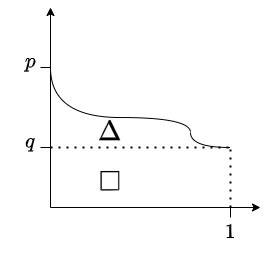
\includegraphics[width=0.5\textwidth]{cdf.drawio.png}
    \caption{The general shape of a loss exceedance function may be split into a sum of a constant function and a reminder as \(\square + \Delta\) and we define \(\widehat{\Delta}\) as the normalized reminder \(\frac{\Delta}{p-q}\) where \(p = p_{\text{attachment}}\), \(q = p_{\text{exhaustion}}\)}
\end{figure}

\printbibliography
\end{document}
